%%%%%%%%%%%%%%%%%%%%%%%%%%%%%%%%%%%%%%%%%%%%%%%%%%%%%%%%%%%%%%%%%%%%%%%%%%%%%%%
%%%%%%%%%%%%%%%%%%%%%%%%%%%%%%%%%%%%%%%%%%%%%%%%%%%%%%%%%%%%%%%%%%%%%%%%%%%%%%%
% CONTRIBUTION TO THE MESONH BOOK1: "Atmospheric chemistry"
% file:    chimie.tex
% created: Fri Nov  5 13:38:33 CET 1999
% author:  Celine Mari/Pierre Tulet/Karsten Suhre
% purpose: book1 for MesoNH
%%%%%%%%%%%%%%%%%%%%%%%%%%%%%%%%%%%%%%%%%%%%%%%%%%%%%%%%%%%%%%%%%%%%%%%%%%%%%%%
%
%\begin{document}
%
\chapter{Atmospheric Chemistry}
\minitoc
%\chapter{Scientific documentation}
%
This chapter reviews the main processes for the gas phase chemistry.

%%%%%%%%%%%%%%%%%%%%%%%%%%%%%%%%%%%%%%%%%%%%%%%%%%%%%%%%%%
%%% DRY DEPOSITION (P. Tulet) modif (G. Guenais 02/02/01)
%%%%%%%%%%%%%%%%%%%%%%%%%%%%%%%%%%%%%%%%%%%%%%%%%%%%%%%%%%
\section{Dry deposition of gaseous species}

The removal of gases from the atmosphere by turbulent transfer and uptake at
the surface is defined as dry deposition. This process enables some
chemically reactive gases to be efficiently removed from the atmosphere. 
Dry deposition of gaseaous specied was introduced in Meso-NH by 
\citet{Tulet2003}.
Dry deposition is usually parametrized through a deposition velocity \vd,
defined by \vd$=-\frac{F_c}{c(z)}$, where $F_c$ is the flux of the considered
compound ($F_c$ is assumed constant over the considered range of heights) and
$c(z)$ is the concentration at height $z$ (molecules/cm$^3$). \vd~ depends
on many variables such as wind speed, temperature, radiation, the considered
species and the surface conditions. It is commonly described
through a resistance analogy often called "Big-Leaf" Model 
\citep[e.g.][]{Wesely1977}.
\[
v_d(z)=\frac{1}{R_a+R_b+R_c}\]
where $R_a$ is the aerodynamic resistance, which is a function of the
turbulence 
in the boundary layer, $R_b$ the quasi-laminar resistance partially controlled
by molecular diffusion, and $R_c$ the surface
resistance, which combines all the transfer pathways playing a role in the
uptake of trace gases by the surface.

\begin{figure}[htb]
\centerline{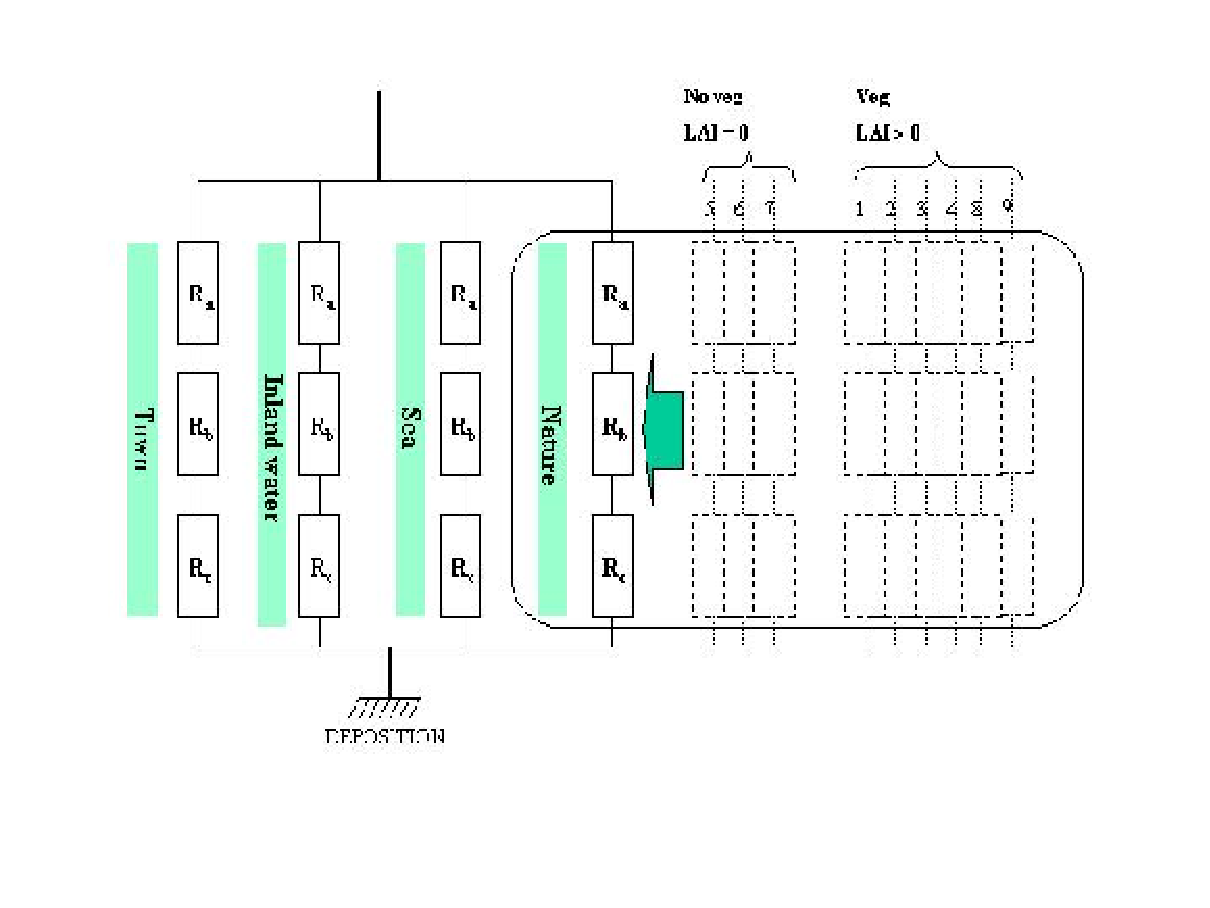
\includegraphics[width=0.5\textwidth]{\EPSDIR/schema_dep.pdf}}
%\centerline{\psfig{file=\EPSDIR/schema_dep.epsi,width=0.5\textwidth}}
%\centerline{\psfig{file=../DEPOT/schema_dep.epsi,width=0.5\textwidth}}
\caption{\sl ~{Schematic resistances for dry deposition module in
accordance with the surface state. 
Ra represents the aerodynamic resistance, Rb the quasi-laminar
resistance and Rc the surface resistance.}}
\label{schema} 
\end{figure}
%&&&&&&&&&&&&&&-------------GG0------------------
\subsubsection*{Meso-NH surface for dry deposition}
As shown in Fig. \ref{schema}, earth surface is divided into four major
parts. On those surfaces calculation of specific parameters are done
(friction velocities, surface resistances, ...). The earth splitting
is done as follows : town horizontal fraction \citep{Masson2000}, inland
water and sea surfaces (differents because of their surface
temperature) and nature fractions. Nature surface is cut into 9 cover type, 
which can be reorganized by 'patches' (1 to 9). 
One 'patch' contains one or several cover types (user choice). 
These cover types are connected with the Wesely classes of
vegetation for the surface resistance data parameters (see Table
\ref{classveg}).
\begin{table}
\begin{center}
\begin{tabular}{|l|l|} \hline
\bf{Meso-NH nature cover type} & \bf{Wesely correspondence class} \\ \hline 
 C3 cultures types(low) &       (2) Agricultural land \\ 
 C4 cultures types(hight)&      (2) Agricultural land \\ 
 forest and trees       &       (4) Deciduous and (5) coniferous
 forest \\ 
 grassland              &       (3) Range land \\ 
 no vegetation (smooth) &       (8) Baren land, mostly desert \\  
 no vegetation (rocks)  &       (11) Rocky open areas with low-growing
 shrubs \\ 
 permanent snow and ice &        No correspondence \\ 
 irrigated crops        &       (9) None forested wetland \\ 
 irrigated parks gardens or peat bogs   & (6) Mixed forest including
 weet land\\
                        &                  and (9) none forest wetland \\ 
\hline
\end{tabular}
\caption{\sl ~{Meso-NH vegetative cover type and Wesely connected
class for dry deposition calculation}}
\label{classveg}
\end{center}
\end{table}

%&&&&&&&&&&&&&&-------------GG0------------------

\subsection{Resistances for dry deposition}
\subsubsection*{Aerodynamic resistance $R_a$}

$R_a$ determines the rate of transport of gases between a given level in the
\atm~and the height of the effective surface sink. 
It is usually calculated as the bulk aerodynamic resistance to the transfer of
momentum :  $R_a(z_R)=\frac{1}{\bf{C_D} \bf{V_A}}$, where $\bf{C_D}$ is the drag
coefficient for momentum
\citep[see for example][]{Wesely1977,Sheih1979,Walcek1986}
and $\bf{V_A}$ the wind speed (in the following, the parameters which are
already used or calculated in the MESO-NH subroutines will be noted in bold
characters).
%-------------------------GG1
% The $\bf{C_D}$ coefficient is calculated in the ISBA scheme.
%-------------------------GG1
The reference height $z_R$ is taken as the lowest atmospheric level in
the ISBA scheme.
\medskip

An alternate way is to use the ISBA calculation of $\bf {R_a}$,
$\bf{R_a(z_R)}=\frac{1}{\bf{C_H} \bf{V_A}}$ 
which determines the transfer of water
vapor. $\bf{C_H}$ is then the drag coefficient depending upon the thermal
stability of the \atm~.  \\
%--------------------------GG2
Heat drag coefficients are calculated in WATER\_FLUX for inland water
and sea, in URBAN for artificial land (town) and in ISBA for the other 
nature cover types or patch. So there is one $\bf {R_a}$ different for
each different coefficient.
\\
This formulation of $\bf {R_a}$ requires an additional term to the
quasi-laminar resistance described below.
%--------------------------GG2
\subsubsection*{Quasi-laminar resistance $R_b$}

The component $R_b$ is associated with transfer through the quasi-laminar 
layer in contact with the surface. $R_b$ quantifies the way in which pollutant
or heat transfer differ from momentum transfer in the immediate vicinity of the
surface (this is due to the effects of molecular diffusion and the difference 
of roughness lengths found for momentum and mass transfer). 
$R_b$ depends on both turbulence characteristics and the molecular
diffusion of the considered gas. Transport of a gas through the
quasi-laminar layer by molecular diffusion depends on the thickness of the
layer, the concentration gradient over the layer and on a diffusion constant,
which in turn depends on the radius of the gas molecule and on the temperature.
The complexity of vegetation generally limits the accuracy with which the
magnitude of this mechanism can be estimated in the field. This resistance can
be conveniently written as:
\[ R_b=\frac{1}{k u^*} \log (\frac{z_0}{z_c})\]
$k$ is the Von Karman constant and $u^*$ the friction velocity.
$z_c$ is the roughness length for the pollutant under investigation (Baldocchi
et al., 1987). 

According to \citet{Hicks1987,Garrat1973}
$R_b$ can be approximated for vegetation and fibrous roughness elements by :
\[ R_b = \frac{2}{\bf{k} \bf{u^*}}(\frac{Sc}{Pr})^{2/3} \]
$Sc$ and $Pr$ are the Schmidt and Prandtl numbers respectively.
$Pr=0.72$ and $Sc=\frac{\nu}{D_i}$, with $\nu$ the kinematic viscosity of
air (0.15 cm$^2$s$^{-1}$, 20$^\circ$ C, p = 1atm) and $D_i$ the molecular
diffusivity of gas $i$ (see table \ref{const} for some of these
constants). 
%----------------GG3------------------
For snow, ice, water and bare soil, $R_b$ can be calculated by
\citet{Ganzeveld1995}:\[ R_b =
\frac{1}{\bf{k} \bf{u^*}}(\frac{Sc}{Pr})^{2/3} \]\\
This formulation is used for all Meso-NH grid fraction cover with no
vegetation (Leaf Area Index = 0), that include artificial land, water
and sea.\\
Definition of friction velocity in MNH is given by : $u^* =
\sqrt[4]{{\bf {<u'w'>}_{xx}}^2+{\bf{<v'w'>}_{xx}}^2}$. Where $<u'w'>_{xx}$ and
$<v'w'>_{xx}$ represents   
surface fluxes of horizontal momentum in x and y directions (xx for sea,
water, town and nature patch).
%----------------GG3------------------
Molecular diffusivity species/air  can be obtain by the knowledge of $H_2O/air$ diffusivity.
The coefficient of diffusivity is given by the general formula as:\\
$D = v l /3 = 0.376 k T \, / (N (M Cste)^{0.5})$\\
with
l mean free path,
v mean molecular velocity,
k Boltzmann constant,
T temperature,
N concentration,
M molecular mass.
So we use for computing molecular diffusivity: \\ 
$$
D(gaz)=D(H_2O) \left(\frac{M(H_2O)}{M(gaz)} \right)^{0.5}
$$
with 
$$
D(H_2O)= 2.22e-5 + 1.25 10^{-7} (T + 273)  for 193 K < T < 0 K
$$
$$
D(H_2O)= 2.22e-5 + 1.46 10^{-7} (T + 273)  for 273 K < T < 323 K 
$$

\medskip

However, these formulations of $R_b$ remain still controversial. 
Recent results from fields studies 
indicate that they
are not in agreement with experimentally derived results, at least
for the transfer of HNO$_3$
over wheat \citep{Muller1993}.
%-----------GG4--------------------
At last, velocity dry deposition is not very sensitive of the choosen
definition of $R_b$ \citep{Ganzeveld1995}.
%-----------GG4--------------------
\subsubsection*{Surface Resistance $R_c$}

The surface resistance is the most difficult of the three resistances to
describe. $R_c$ values can be obtained from theoretical considerations based
for instance on solubility and equilibrium; calculations in combination with
simulation of vegetation specific processes, such as accumulation, transfer
process through stomata, mesophyll, cuticles, etc $\ldots$
\citep{Baldocchi1987,Wesely1989}. The values of $R_c$ are based on
measurements of $V_d$. By determining $R_a$ and $R_b$ from the meteorological
measurements, $R_c$ is calculated as the residual resistance. The calculated
$R_c$ are then related to surface conditions, time of day, etc $\ldots$ in
order to obtain parametrizations of $R_c$.

\begin{figure}[htb]
%\centerline{\psfig{file=../DEPOT/surf.epsi,width=0.4\textwidth}}
%\centerline{\psfig{file=\EPSDIR/surf.epsi,width=0.4\textwidth}}
\centerline{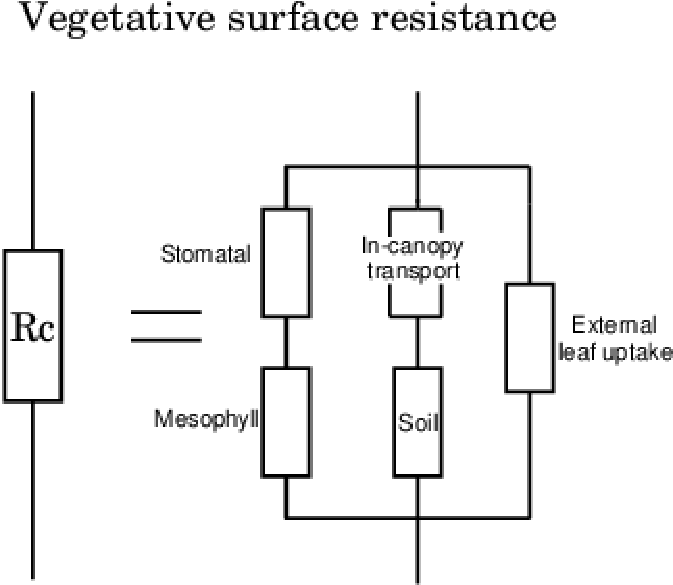
\includegraphics[width=0.4\textwidth]{\EPSDIR/surf.pdf}}
\caption{\sl ~{Surface resistance schematic for vegetation.}}
\label{schema2}
\end{figure}
%-------------GG5-------------------------------
$R_c$ is a function of the canopy stomatal resistance $R_{stom}$ and mesophyll
resistance $R_m$, the canopy cuticle or external leaf resistance $R_{ext}$, the
soil resistance $R_{soil}$ and in-canopy resistance $R_{inc}$, 
and the resistance
to surface waters or moorland pools, $R_{wat}$, $R_{sea}$ \citep{Erisman1994}
In turn, these resistances are affected by leaf area index, stomatal
physiology, soil and external leaf surface, pH presence and chemistry of
liquid drops and films.
In summary, $R_c$ should be calculated as \cite{Erisman1994}:
\begin{itemize}
%\item {Vegetative surfaces :
%\[R_c={\left(\frac{1}{R_{stom}+R_m}+\frac{1}{R_{inc}+R_{soil}} +
%\frac{1}{R_{ext}} \rigth) }^{-1} \]}  
%\item {Water surfaces : \[R_c=R_{wat}\]}
%\item {Sea surfaces : \[R_c=R_{sea}\]}
%\item {Bare soil (no vegetation) : \[R_c=R_{no}\]}
%\item {Rock surfaces : \[R_c=R_{rock}\]}
%\item {Snow/ice  cover : \[R_c=R_{snow}\]}
%\item {Artificial land : \[R_c=R_{town}\]}
\item Vegetative surfaces :
$
R_c= \left(\frac{1}{R_{stom}+R_m}+\frac{1}{R_{inc}+R_{soil}} + \frac{1}{R_{ext}} \right)^{-1} 
$
\item Water surfaces : $R_c=R_{wat}$
\item Sea surfaces : $R_c=R_{sea}$ 
\item Bare soil (no vegetation) : $R_c=R_{no}$
\item Rock surfaces : $R_c=R_{rock}$
\item Snow/ice  cover : $R_c=R_{snow}$
\item Artificial land : $R_c=R_{town}$

\end{itemize}
%-------------GG5-------------------------------
\subsubsection*{Stomatal and mesophyll resistance $R_{stom}$ and $R_m$}

The stomatal resistance for water vapor is calculated in the ISBA subroutines
as \[ \bf{R_{stom}}=\frac{R_{smin}}{F_1 F_2 F_3 F_4\, LAI},\] where
$\bf{LAI}$ is the leaf area index computed by patch, and $F_1$, $F_2$,
$F_3$, $F_4$ are limiting factors depending on 
radiation, wetness of soil and temperature. In order to describe the stomatal
resistance for another gas, the ISBA $\bf{R_{stom}}$ for water vapor should be
corrected as followed :
\[ R_{stom,x}={\bf{R_{stom}}} \times \frac{D_{H_2O}}{D_x},\]
$D_{H_2O}$ and ${D_x}$ are the diffusion coefficients of $H_2O$ and $x$
respectively \citep{Wesely1989}.

\medskip

There is not much knowledge on the mesophyll resistance for different gases and
the conditions which determine its value. For some gases, such as SO$_2$ %3.e-2
O$_3$ %1.e-2
and NH$_3$, %1.5e-1
$R_m$ is experimentally found near zero values \citep{Erisman1994}.
This is in agreement with the parametrization suggested by \cite{Wesely1989}
for the calculation of the mesophyll resistance:
\[ R_{mx} = ( \frac{H^*}{3000} + 100 f_0) ^{-1} \] 
In this expression, $H^*$ is the Henry's law constant for the considered gas,
$f_0$ a reactivity factor which determines the rate of reduction of the
substance. Two parallel pathways are thus assumed, one for highly reactive
gases, the other one for soluble substances. Table \ref{const} 
lists $H^*$ and
$f_0$ for some species \citep{Baer1992}.

\begin{table}
\begin{center}
\begin{tabular}{lll} \hline
Species         & Reactivity factor     & Henry's law (M/atm) \\ \hline 
Sulfur dioxide  & 0     & $1.6(1+2.1\; 10^{-2}/H+)$ \\
Nitric oxide    & 0     & $1.9\; 10^{-3}$        \\
Nitrogen dioxide & 0.1  & $10^{-2}$              \\
Nitric acid      & 0    & $5.8\; 10^{6}/H+$       \\
Ozone           & 1.    & $1.5\; 10^{-2}$         \\
Hydrogen peroxide  & 0  & $1.8\; 10^{5}$          \\
Formaldehyde    & 0     & $3.26\; 10^{-4}$ \\
Aldehydes       & 0     & $76$ \\
Organic acids   & 0     & $1.45\; 10^{-4}$ \\
Organic peroxide  & 0.25& $665$ \\
Peroxyacetic acid  & 0.5& $1635$ \\
Peroxyacetyl nitrate &0.1& $3.6$ \\
Other alkanes & 0       & $1.\; 10^{-3}$ \\
Ethane           & 0    & $1.9\; 10^{-3}$ \\
Ethene           & 0    & $4.9\; 10^{-3}$ \\
Propene           & 0   & $4.7\; 10^{-3}$ \\
Butene and other olefins  & 0   & $1.3\; 10^{-3}$ \\
Toluene       & 0       & $0.15$ \\
Xylene      & 0         & $0.1$ \\ 
\hline
\end{tabular}
\caption{\sl ~{Reactivity factor and Henry's law constants for different chemical species}}
\label{const}

\end{center}
\end{table}

\subsubsection*{External leaf uptake $R_{ext}$}

The external leaf uptake can act as an effective sink, especially for soluble
gases at wet surfaces. 
%----------------GG6---------------------
The resistance of the outer surfaces in the upper canopy (leaf cuticular
resistance in healthy vegetation) is computed by \cite{Wesely1989}, for a
dry surface to any gas (x), as:
\[R_{ext.x.dry}=R_{ext}(10^{-5}H^*+f_0)^{-1}\]
In this expression, $R_{ext}$ is given by land category and season in table
\ref{resdebase},  the constants ($H^*$, $f_0$) can be found in table 
\ref{const}.\\
The following equation is supposed to give an analytic expression of
$\bf{R_{ext}}$ in accordance with Wesely table \ref{resdebase}, and 
including seasonal variations through the leaf area index $\bf LAI$:
\[R_{ext}=6000 - 4000 \tanh(1.6( {\bf{LAI}} -1.6))\]
These results had been compared with Wesely table in accordance with 
Méso-NH (ISBA) data of LAI (see Fig. \ref{lai_rext}).
\begin{figure}
%\centerline{\psfig{file=../DEPOT/rext_lai.epsi,width=0.5\textwidth}}
%\centerline{\psfig{file=\EPSDIR/rext_lai.epsi,width=0.5\textwidth}}
\centerline{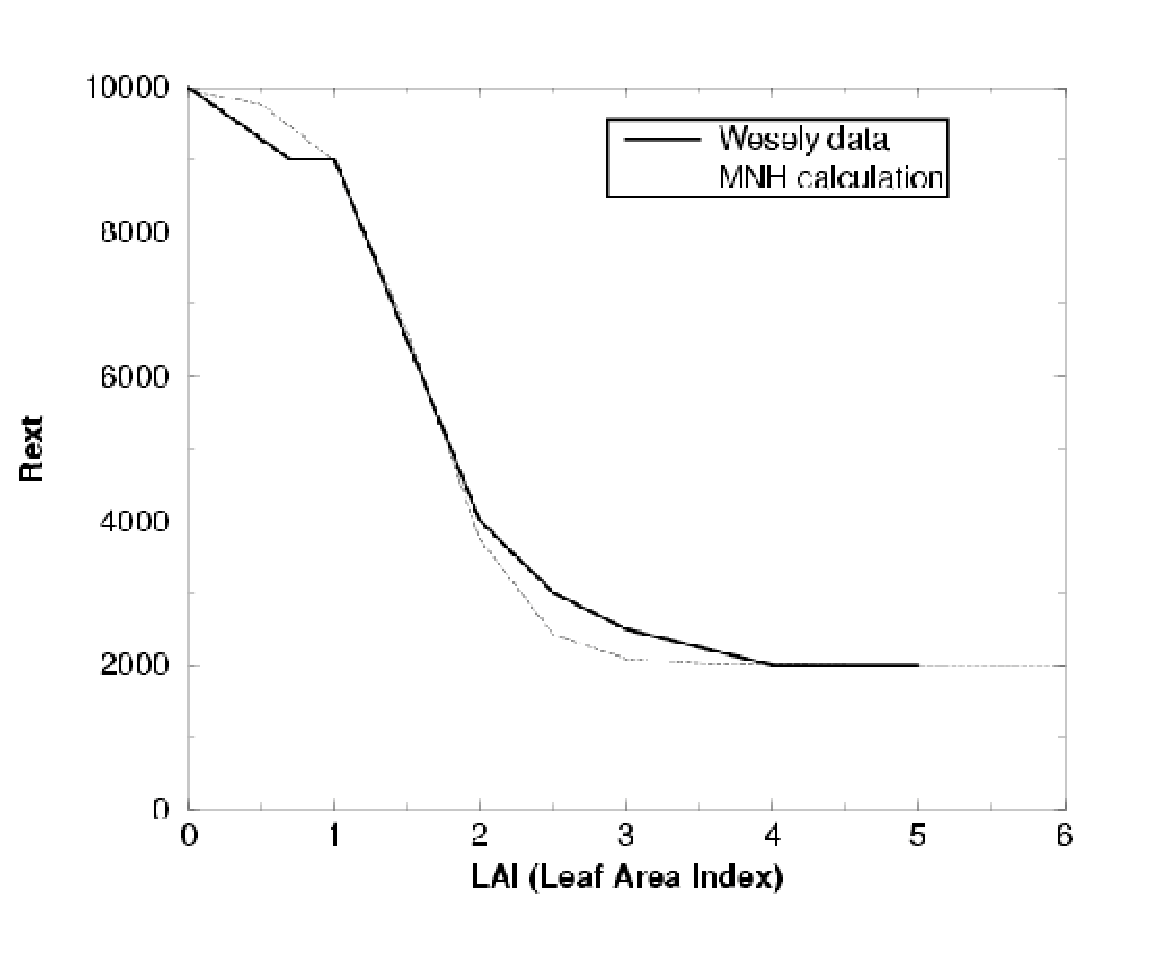
\includegraphics[width=0.5\textwidth]{\EPSDIR/rext_lai.pdf}}
\label{lai_rext}
\caption{\sl{$\bf{R_{ext}}$ fonction of $\bf{LAI}$ (from Wesely table)}}
\end{figure}

\begin{table}
\begin{center}
\begin{tabular}{lllllllllll}
\hline
1&2&3&4&5&6&7&8&9&10&11 \\ \hline
\multicolumn{11}{l}{Midsummer with lush vegetation}\\
9999 & 2000& 2000&   2000   & 2000  & 2000  & 9999 & 9999 & 2500 & 2000 & 4000
\\
\multicolumn{11}{l}{Autumn with unharvested cropland}\\
9999 & 9000& 9000&   9000   & 4000  & 8000  & 9999 & 9999 & 9000 & 9000 & 9000
\\
\multicolumn{11}{l}{Late autumn after frost, no snow}\\
9999 & 9999 & 9000&   9000   & 4000  & 8000  & 9999 & 9999 & 9000 & 9000 & 9000
\\
\multicolumn{11}{l}{Winter}\\
9999 & 9999 & 9999 & 9999 & 6000  & 9000  & 9999 & 9999 & 9000 & 9000 & 9000
\\
\multicolumn{11}{l}{Spring}\\
9999 & 4000& 4000&   4000   & 2000  & 3000  & 9999& 9999&  4000 & 4000 & 8000
\\ \hline
\end{tabular}
\caption { \sl~{Input resistances for calculation of external leaf resistance
(Wesely 1989) : (1) urban land, (2) agricultural land, (3) range land,
(4) deciduous forest, (5) coniferous forest, (6) mixed forest
including wetland, (7) water, (8) barren land, mostly desert,
(9) nonforested wetland, (10) mixed agricultural and range land,
(11) rocky-open areas with low-growing shrubs}} 
\label{resdebase}

\end{center}
\end{table}

In case of dew or rain, and according to the same author and
\citep{Walmsley1996}, the equation should be replaced by :
\[R_{ext.x.wet}=[1/(3R_{ext.x.dry})+(10^{-7}H^*+f_0/R_{extOzone}]^{-1}\]
with

\begin{itemize}
 
\item { Rain: \[ R_{extOzone} = (1/(3R_{ext})+1/1000 )^{-1}\]  }
 
\item { Dew: \[ R_{extOzone} = (1/(3R_{ext})+1/3000 )^{-1}\]  }
\end{itemize}
 
To apply the same comput for each species we approximate in case of
wet soil these formulas by 
using $R_{extOzone}$ as 3000 s/m.

These formulas should be corrected when surface
temperature decreases below -2$^\circ$C by adding the value
$1000 \exp (-T-4)$, in order to take into acccount the lesser uptake
by surfaces 
when cold.
%----------------GG6---------------------
\subsubsection*{In-canopy transport $R_{inc}$}

Deposition to soils under vegetation can be relatively important. 
\cite{Meyers1988} found that 20\% - 30\% of SO$_2$ was deposited 
in summer to the soil under a deciduous forest.
This transport is due to large-scale intermittent eddies through the
vegetation. 
The corresponding resistance has been parametrized by \cite{Erisman1994}
using data of \cite{vanPul1994}
as:
\[ R_{inc}=\frac{b\; {\bf LAI}\; h}{\bf{u^*}}\]        %LAI_PATCH
$b$ is an empirical constant estimated at 14 $m^{-1}$. $\bf LAI=
LAI\_patch$ is the  
leaf area index given by patches computed in the GROUND\_PARAMn files
and $\bf h$ is the 
vegetation height which can be calculated as four times the 
vegetation roughness length
(formula of \cite{Kondo1986}, assuming a dense vegetation canopy
with similar height).

\medskip
%----------------GG7---------------------
\subsubsection*{Soil resitances for surfaces with no vegetation and those
under vegetation}
Table \ref{rsol} presents a review of soil resistances for SO$_2$ and O$_3$
for clay, sand, snow and it is completed
with Table \ref{rcsoil}, Wesely value for all other vegetation types, 
town and rock.\\
For other gases, the resistance can be computed following \cite{Wesely1989} :
\[ R_{soilx} = (\frac{H^*}{10^5 R_{soilSO_2}}+ \frac{f_0}{R_{soilO_3}})^{-1} \]
According to the same author, this formula should be corrected when surface
temperature decreases below -2$^\circ$C by adding the value :
\[R_{soilx} =  R_{soilx} + 1000 \exp (-T-4) \]
For no vegetation cover soil surface composition
(sand, clay) is considered. If it is 
covered by snow, this formlation will be update by using Table \ref{rsol}. 
\[ R_{sandx} = (\frac{H^*}{10^5 R_{sandSO_2}}+ \frac{f_0}{R_{sandO_3}})^{-1} \]
\[ R_{clayx} = (\frac{H^*}{10^5 R_{claySO_2}}+ \frac{f_0}{R_{clayO_3}})^{-1} \]
\[ R_{snowx} = (\frac{H^*}{10^5 R_{snowSO_2}}+ \frac{f_0}{R_{snowO_3}})^{-1} \]
In this context $R_{no.x}$ for bare ground (no veg.) without snow is
the weighted average of $R_{sandx}$ and $R_{clayx}$ as: 
$$ R_{no.x} = ( \frac{\alpha_{sand}}{R_{sandx}} +
                \frac{\alpha_{clay}}{R_{clayx}} )^{-1} $$
with\\
$\alpha_{sand}$ : percentage of sand in the ground \\
$\alpha_{clay}$ : percentage of clay in the ground \\
For all the other type of soil, resistance is calculated with Table
\ref{rcsoil} as:
\begin{eqnarray*} 
R_{rockx} & = & (\frac{H^*}{10^5 R_{rockSO_2}}+
        \frac{f_0}{R_{rockO_3}})^{-1}  \\
R_{townx} & = & (\frac{H^*}{10^5 R_{townSO_2}}+
        \frac{f_0}{R_{townO_3}})^{-1} \\
R_{c3x} & = & (\frac{H^*}{10^5 R_{c3SO_2}}+ \frac{f_0}{R_{c3O_3}})^{-1} \\
R_{c4x} & = & (\frac{H^*}{10^5 R_{c4SO_2}}+ \frac{f_0}{R_{c4O_3}})^{-1} \\
R_{treex} & = & (\frac{H^*}{10^5 R_{treeSO_2}}+
        \frac{f_0}{R_{treeO_3}})^{-1} \\
R_{grassx} & = & (\frac{H^*}{10^5 R_{grassSO_2}}+
        \frac{f_0}{R_{grassO_3}})^{-1} \\
R_{irrx} & = & (\frac{H^*}{10^5 R_{irrSO_2}}+
        \frac{f_0}{R_{irrO_3}})^{-1} \\
R_{parkx} & = & (\frac{H^*}{10^5 R_{parkSO_2}}+
        \frac{f_0}{R_{parkO_3}})^{-1} \\
\end{eqnarray*}

\begin{table}
\begin{center}
\begin{tabular}{lll}\hline
Type of soil & SO$_2$                    & O$_3$  \\ \hline
snow           & 540 at T $ < $-1$^o$C      & 2000   \\ 
               & 70(2-T) at -1 $<$ T $<$ 1 &        \\ 
sand           & 1000                      & 200    \\ 
clay           & 1000                      & 100    \\  \hline
\end{tabular}
\caption{\sl ~{Soil resistance}}
\label{rsol}
\end{center}
\end{table}

\begin{table}
\begin{center}
\begin{tabular}{llllllllll}\hline
\multicolumn{10}{l}{MNH cover type}\\
 c3 & c4 & tree & grass & no & rock & snow/ice & irr & park & town \\ 
\hline
\multicolumn{10}{l}{Soil resistance for SO$_2$}\\
150 & 150 & 500 & 350 & 1000 & 400 & no data & 0 & 100 & 400 \\
\hline
\multicolumn{10}{l}{Soil resistance for O$_3$}\\
150 & 150 & 200 & 200 & 400 & 200 & no data & 1000 & 700 & 300 \\
\hline  
\end{tabular}
\caption{\sl ~{Soil resistance for MNH-C decomposition from Wesely
table (quasi constant during the year). Values for ``snow/ice'' and
``no'' (no veg.) are not used see Table \ref{rsol}.}} 
\label{rcsoil}
\end{center}
\end{table}

\subsubsection*{Surfaces resistances for sea and water}
For deposition over water surface bodies, the surface resistance can
be calculated from the expression recommended by \cite{Sehmel1980} that
incorporates wind speed and 
and air/water partitioning coefficient, rather than from Wesely's
tabulated values for water bodies. The surface resistance over water
is: 

\[R_{waterx} = \frac{2,54 . 10^{-4}}{H^* \bf{T_{water}} u_*}  = Rc_{waterx}\] 
\[R_{seax} = \frac{2,54 . 10^{-4}}{H^* \bf{T_{sea}} u_*}  = Rc_{seax}\]
 
\subsection{Dry deposition velocity formulation}

\subsubsection*{Artificial land resistance}
$$ Rglobal^{town} = Ra^{town} + Rb^{town} + Rc^{town} $$
\subsubsection*{Sea and water resistance}
$$Rglobal^{water} = Ra^{water} + Rb^{water} + Rc^{water}$$\\
$$Rglobal^{sea} = Ra^{sea} + Rb^{sea} + Rc^{sea}$$
\subsubsection*{Nature final resistance}
$$ Rglobal^{nature} = \sum_{i=1}^{nvegtype} {\left(
\frac{\alpha_i}{Ra^{j_{patch}} + Rb^{j_{patch}} + Rc^{i} }\right)^{-1}} $$
with\\
$i \stackrel{f}{\longmapsto} f(i) = j_{patch}$ like
 $i \in [1,nvegtype]$, $f(i)=j_{patch} \in [1,npatch\leq nvegtype]$ \\
and 
 $ \alpha_i $ fraction of cover type (9 types)

\subsubsection*{Dry deposition velocity}

Final dry deposition formulation:
$$
v_{dry deposition} = \frac{\alpha_{water}}{Rglobal^{water}} +
\frac{\alpha_{sea}}{Rglobal^{sea}} +
\frac{\alpha_{townmax}}{Rglobal^{town}} +
\frac{\alpha_{nature}}{Rglobal^{nature}}
$$
where\\ 
\begin{tabbing}
$\alpha_{townmax}$ \=: fraction of town increased \kill
$\alpha_{water}$ \> : fraction of water \\
$\alpha_{sea}$ \> : fraction of sea \\
$\alpha_{townmax}$ \> : fraction of town increased \\
$\alpha_{sea}$ \> : fraction of nature 
\end{tabbing}
Fraction of town has to be increased in order to take account of the non
negligible dry deposition on vertical surfaces in artificial
area. The increase is done as follows:\\
$\alpha_{townmax} = \alpha_{town} (1+2 \frac{H}{L} \, \alpha_{bld})$
with: \\
$\alpha_{town}$ horizontal fraction of town \\
$H$ building height \\
$L$ building caracteristic width \\
$\alpha_{bld}$ fraction of buildings in artificial areas (only)
\begin{figure}[hbp]
%\centerline{\psfig{file=../DEPOT/xbldmax.epsi,width=0.5\textwidth}}
\begin{center}
%\includegraphics[width=15cm,height=5cm]{../DEPOT/xbldmax.epsi}
%\includegraphics[width=15cm,height=5cm]{\EPSDIR/xbldmax.epsi}
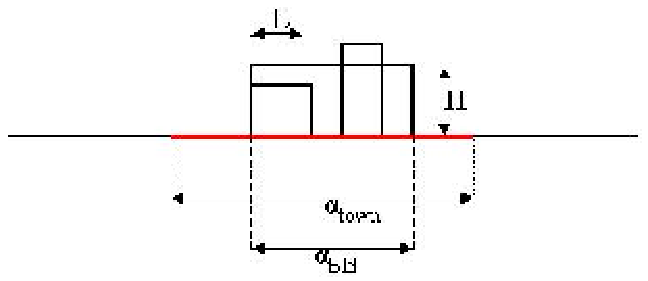
\includegraphics[width=15cm,height=5cm]{\EPSDIR/xbldmax.pdf}
\end{center}
\label{bld}
\caption{\sl{town parameters in MNH (modd\_gr\_field) to increase
fraction of town}} 
\end{figure}
%---------------------GG8---------------

%%%%%%%%%%%%%%%%%%%%%%%%%%%%%%%%%%%%%%%%%%%%%%%%%%%%%%%%%%
%%%%%%%%%%%%%%%%%%%%%%%%%%%%%%%%%%%%%%%%%%%%%%%%%%%%%%%%%%
%%%%%%%%%%%%%%%%%%%%%%%%%%%%%%%%%%%%%%%%%%%%%%%%%%%%%%%%%%
%%% PHOTOLYSIS RATES (C. Mari)
%%%%%%%%%%%%%%%%%%%%%%%%%%%%%%%%%%%%%%%%%%%%%%%%%%%%%%%%%%
%%%%%%%%%%%%%%%%%%%%%%%%%%%%%%%%%%%%%%%%%%%%%%%%%%%%%%%%%%
%
%%%%%%%%%%%%%%%%%%%%%%%%%%%%%%%%%%%%%%%%%%%%%%%%%%%%%%%%%%
\section{Photolysis rates}
%%%%%%%%%%%%%%%%%%%%%%%%%%%%%%%%%%%%%%%%%%%%%%%%%%%%%%%%%%
In 1-D version, photolysis rates are calculated on-line using the TUV algorithm 
\linebreak ({\tt http://www.acd.ucar.edu/TUV/ }). 
In 3-D version, a look-up table is calculated 
for clear-sky photolysis rates using TUV model. The look-up table consists 
of photolysis rates at various altitudes, latitudes and hour angles. 
The look-up table is dependant upon the chemical mechanism. 
Within the model, photolysis rates for individual grid cells are interpolated 
from the look-up table. A parameterization is then used to correct the 
clear-sky photolysis rates for cloud cover. 

%----------------------
\subsection{Background}
%----------------------
Many chemical reactions in the atmosphere are initiated by the 
photodissociation of numerous trace gases. These photodissociative reactions are
responsible for most of the smog buildup detrimental to humans, animals, plant 
life and materials. In order to accurately model and predict the effects of air pollution, good photodissociation reaction rate (or photolysis rate) extimates 
must be made. 

Photodissociation is the conversion of solar radiation into chemical energy 
to activate and dissociate chemical species. 
Species that photodissociate include 
many important trace constituents of the troposphere such as $\rm O_3, NO_2, 
HONO, HNO_3, HNO_4, H_2O_2, HCHO, CH_3OOH$ (also see Appendix 1).  The 
simulation accuracy of the entire chemical system is highly dependent upon the
accuracy of photolysis rates, which are the primary sources of radicals in the 
troposphere. Photolysis rates ($\rm min^{-1}$) sometimes called J-values, are 
computed for photodissociation reaction {\it (i)} by
$$
J_i = \int_{\lambda_1}^{\lambda_2} F(\lambda) \sigma_i(\lambda) \Phi_i(\lambda) d\lambda
$$
where, $F(\lambda)$ is the actinic flux (photons $\rm cm^{-2} min^{-1} nm^{-1}$), $\sigma_i(lambda)$ the absorption cross section for the molecule undergoing 
photodissociation ($\rm cm^2 molecule^{-1}$), $\Phi_i(\lambda)$ the quantum 
yield of the photolysis reaction (molecules photon$^{-1}$), and $\lambda$ the 
wavelength (nm). Absorption cross section and quantum yields are functions of 
wavelength,and may also be functions of temperature and pressure; they are 
unique to species and reactions.  Actinic flux is a radiometric quantity that 
measures the spectral radiance integrated over all solid angles per unit area. 
The spherical receiving surface distinguishes the actinic flux from the more 
commonly measured irradiance, which is the radiance falling on a horizontal 
surface. Thus, the actinic flux can be called spherical spectral irradiance. 
The actinic flux changes with time of day, longitude, latitude, altitude, 
and season, and is governed by the astronomical and geometrical relationships 
between the sun and the earth. It is greatly affected by the earth's surface 
albedo as well as by various atmospheric scatterers and absorbers. Hence, 
correct model calculation of the temporal and spatial variation of the 
actinic flux is critical to obtaining accurate photolysis rates for regional 
and mesoscale modeling. 

The current approach includes two stages of processing: (1) a table of clear sky photolysis rates is calculated for specified heights, latitudes and hours 
from local noon, and (2)  photolysis rates are interpolated from the table 
based on grid cell location and the model time, and are corrected for cloud 
cover. This approach is computationally efficient and has been shown by 
\cite{Madronich1987} to give clear-sky photolysis rates within the 
uncertainty of the surface-based measurements.

%-----------------------------
\subsection{Cloud attenuation}
%-----------------------------
The method used to correct for cloud cover is taken from 
\cite{Chang1987} and \cite{Madronich1987}. The correction of 
clear-sky values depends on whether the location is below, above, or 
within the cloud. The below cloud photolysis rate ($\it J_{below}$) is 
calculated as: 
$$
J_{below} = J_{clear} [ 1 + cfrac(1.6 t_r \cos(\theta) - 1) ]
$$
where cfrac is the cloud coverage, $\theta$ is the zenith angle, and $t_r$ 
is the cloud transmissivity. Below cloud photolysis rates will be lower than 
the clear-sky values due to reduced transmission of radiation through 
the cloud. The cloud transmissivity is calculated by:
$$
 t_r = \frac{5-e^{-\tau_{cld}}}{4 + 3 \tau_{cld} (1 - f)}
$$
where f is the scattering phase function asymetry factor (assumed to be 0.86) 
and $\tau_{cld}$ id the cloud optical depth. The cloud 
optical depth equation is derived  from \cite{Stephens1978}: 
$$
log(\tau_{cld}) = 0.2633 + 1.7095\ln[\log(W)]
$$
is only function of liquid path (W), where $\rm W=L\Delta z (g/m^2)$, L is the 
liquid water content ($\rm g/m^3$), and $\Delta$z is the cloud thickness. 
The above cloud top factor ($\rm F_a$) is calculated as:
$$
J_{above} = J_{clear} [1 + cfrac(\alpha_i (1-t_r)\cos(\theta)]
$$
This equation allows for enhancement of photolysis rates above the cloud 
due to the reflected radiation from the cloud. It also includes a reaction 
dependent coefficient ($\alpha_i$) which allows for further above cloud 
enhancements. Within the cloud, the cloud correction factor is a simple 
linear interpolation of the below cloud factor at cloud base to the above 
cloud factor at cloud top. Once computed, the below, above, and within cloud 
factor are used to scale the clear-sky photolysis rates to account for the 
presence of clouds. In the current implementation, all cloud types (including 
clouds composed of ice crystals) are treated the same using the above outlined
procedure.  

%%%%%%%%%%%%%%%%%%%%%%%%%%%% BIBLIOGRAPHY %%%%%%%%%%%%%%%%%%%%%%%%
\begin{btSect}{4-2-GaseousChemistry}
\section{References}
\btPrintCited
\end{btSect}
%%%%%%%%%%%%%%%%%%%%%%%%%%%% BIBLIOGRAPHY %%%%%%%%%%%%%%%%%%%%%%%%
